
\chapter{Anwendung und Algorithmus}

Ziel dieser Arbeit ist es nicht nur eine Methodik zur optische 
Deformationserkennung zu entwickeln, sondern diese Methodik auch in einer 
Anwendung einfach nutzbar zu machen. 

Diese Kapitel dokumentiert diese Anwendung und geht auf Herausforderungen 
in der Entwicklung ein.

\section{Anwendung}

Die Anwendung beeinhaltet verschiedene Funktionen, alle Funktionen 
können separat benutzt werden. Dadurch müssen zeitintensive Vorgänge nicht 
wiederholt werden, sondern Zwischenergebnisse können abgespeichert und 
neu geladen werden. 

Die Anwendung bietet Funktionen um Resultate in dem entsprechenden Dateiformat zu 
speichern. Soweit möglich werden Dateinamen Empfehlungen automatisch ermittelt, 
daher ist es zu empfehlen von Anfang an mit einem einheitlichen Namensschema bei
den 3D-Scannerdaten zu arbeiten. 
Das Schema Bauteilbeschreibung \textunderscore Spannungsstufe 
\textunderscore Scannerdurchlauf.ply
wird empfohlen. Ein Beispiel für die zweite Pointcloud eines FDM-Bauteil bei der
vierten Spannungsstufen wäre also "FDM0\textunderscore SP4\textunderscore 2.ply"


\begin{figure}[H]
    \centering
    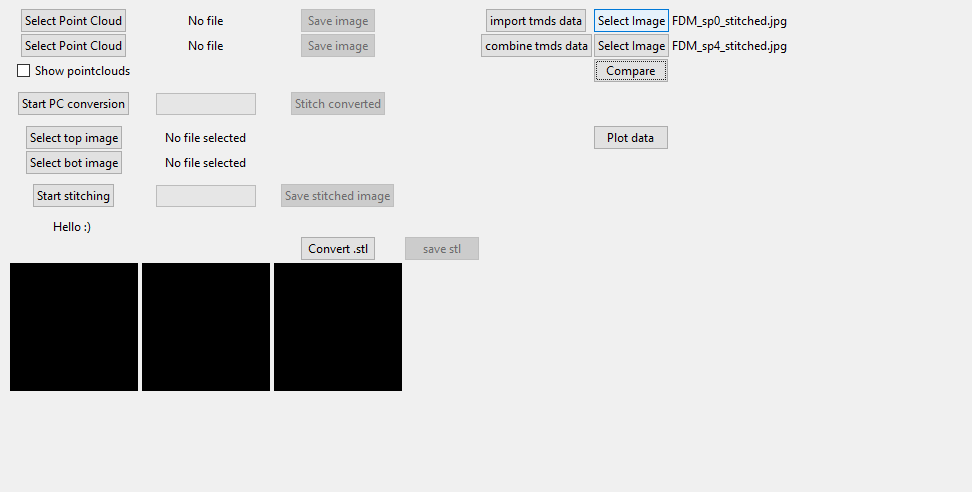
\includegraphics[width=0.5\textwidth]{images/software_screenshot.png}
    \caption{Anwendungsoberfläche}
    \label{fig:software_screenshot}
\end{figure}

[Hier will ich noch auf die folgenden Dinge eingehen:]

\begin{itemize}
    \item Alle Buttons und Displays erklären
    \item Nebenläufigkeit (Threads) um Prozesse wie das Laden von Pointclouds 
    zu verschnellern.
    \item  python -> c code um arbeiten in Arrays und mit großen Daten zu verschnellern
    (Vergleich Laufzeit ca. 10fach schneller)
\end{itemize}


